\section{Steps in the Production Line}
The planned production line consists of several steps that can be seen in figure \ref{fig:ProdLineSchem}. A visual representation from the simulation with Visual Components can be found in figure \ref{fig:ProdLineVisComp}.

\begin{figure}[H]
	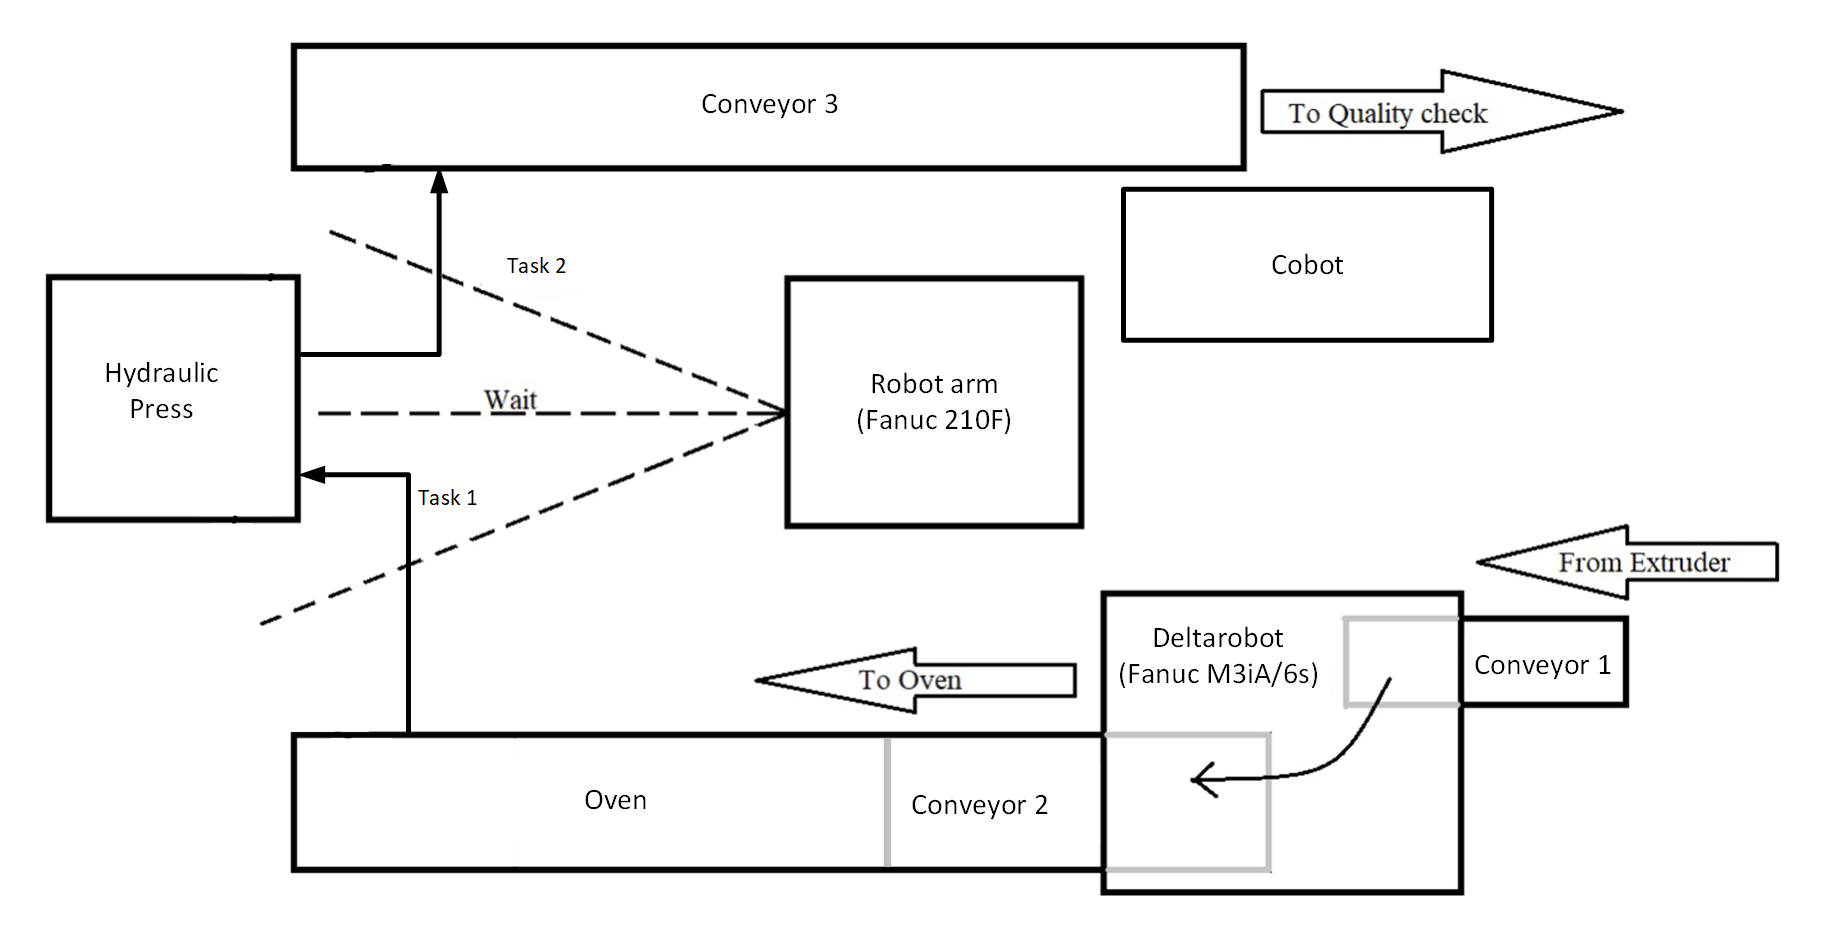
\includegraphics[
	width=\linewidth,
	center,
	keepaspectratio,
	]{ProductionLineSetup/drawing}
	\caption{Schematic of the floorplan \cite{AliyaThesis}}
	\label{fig:ProdLineSchem}
\end{figure}

\begin{figure}[h]
	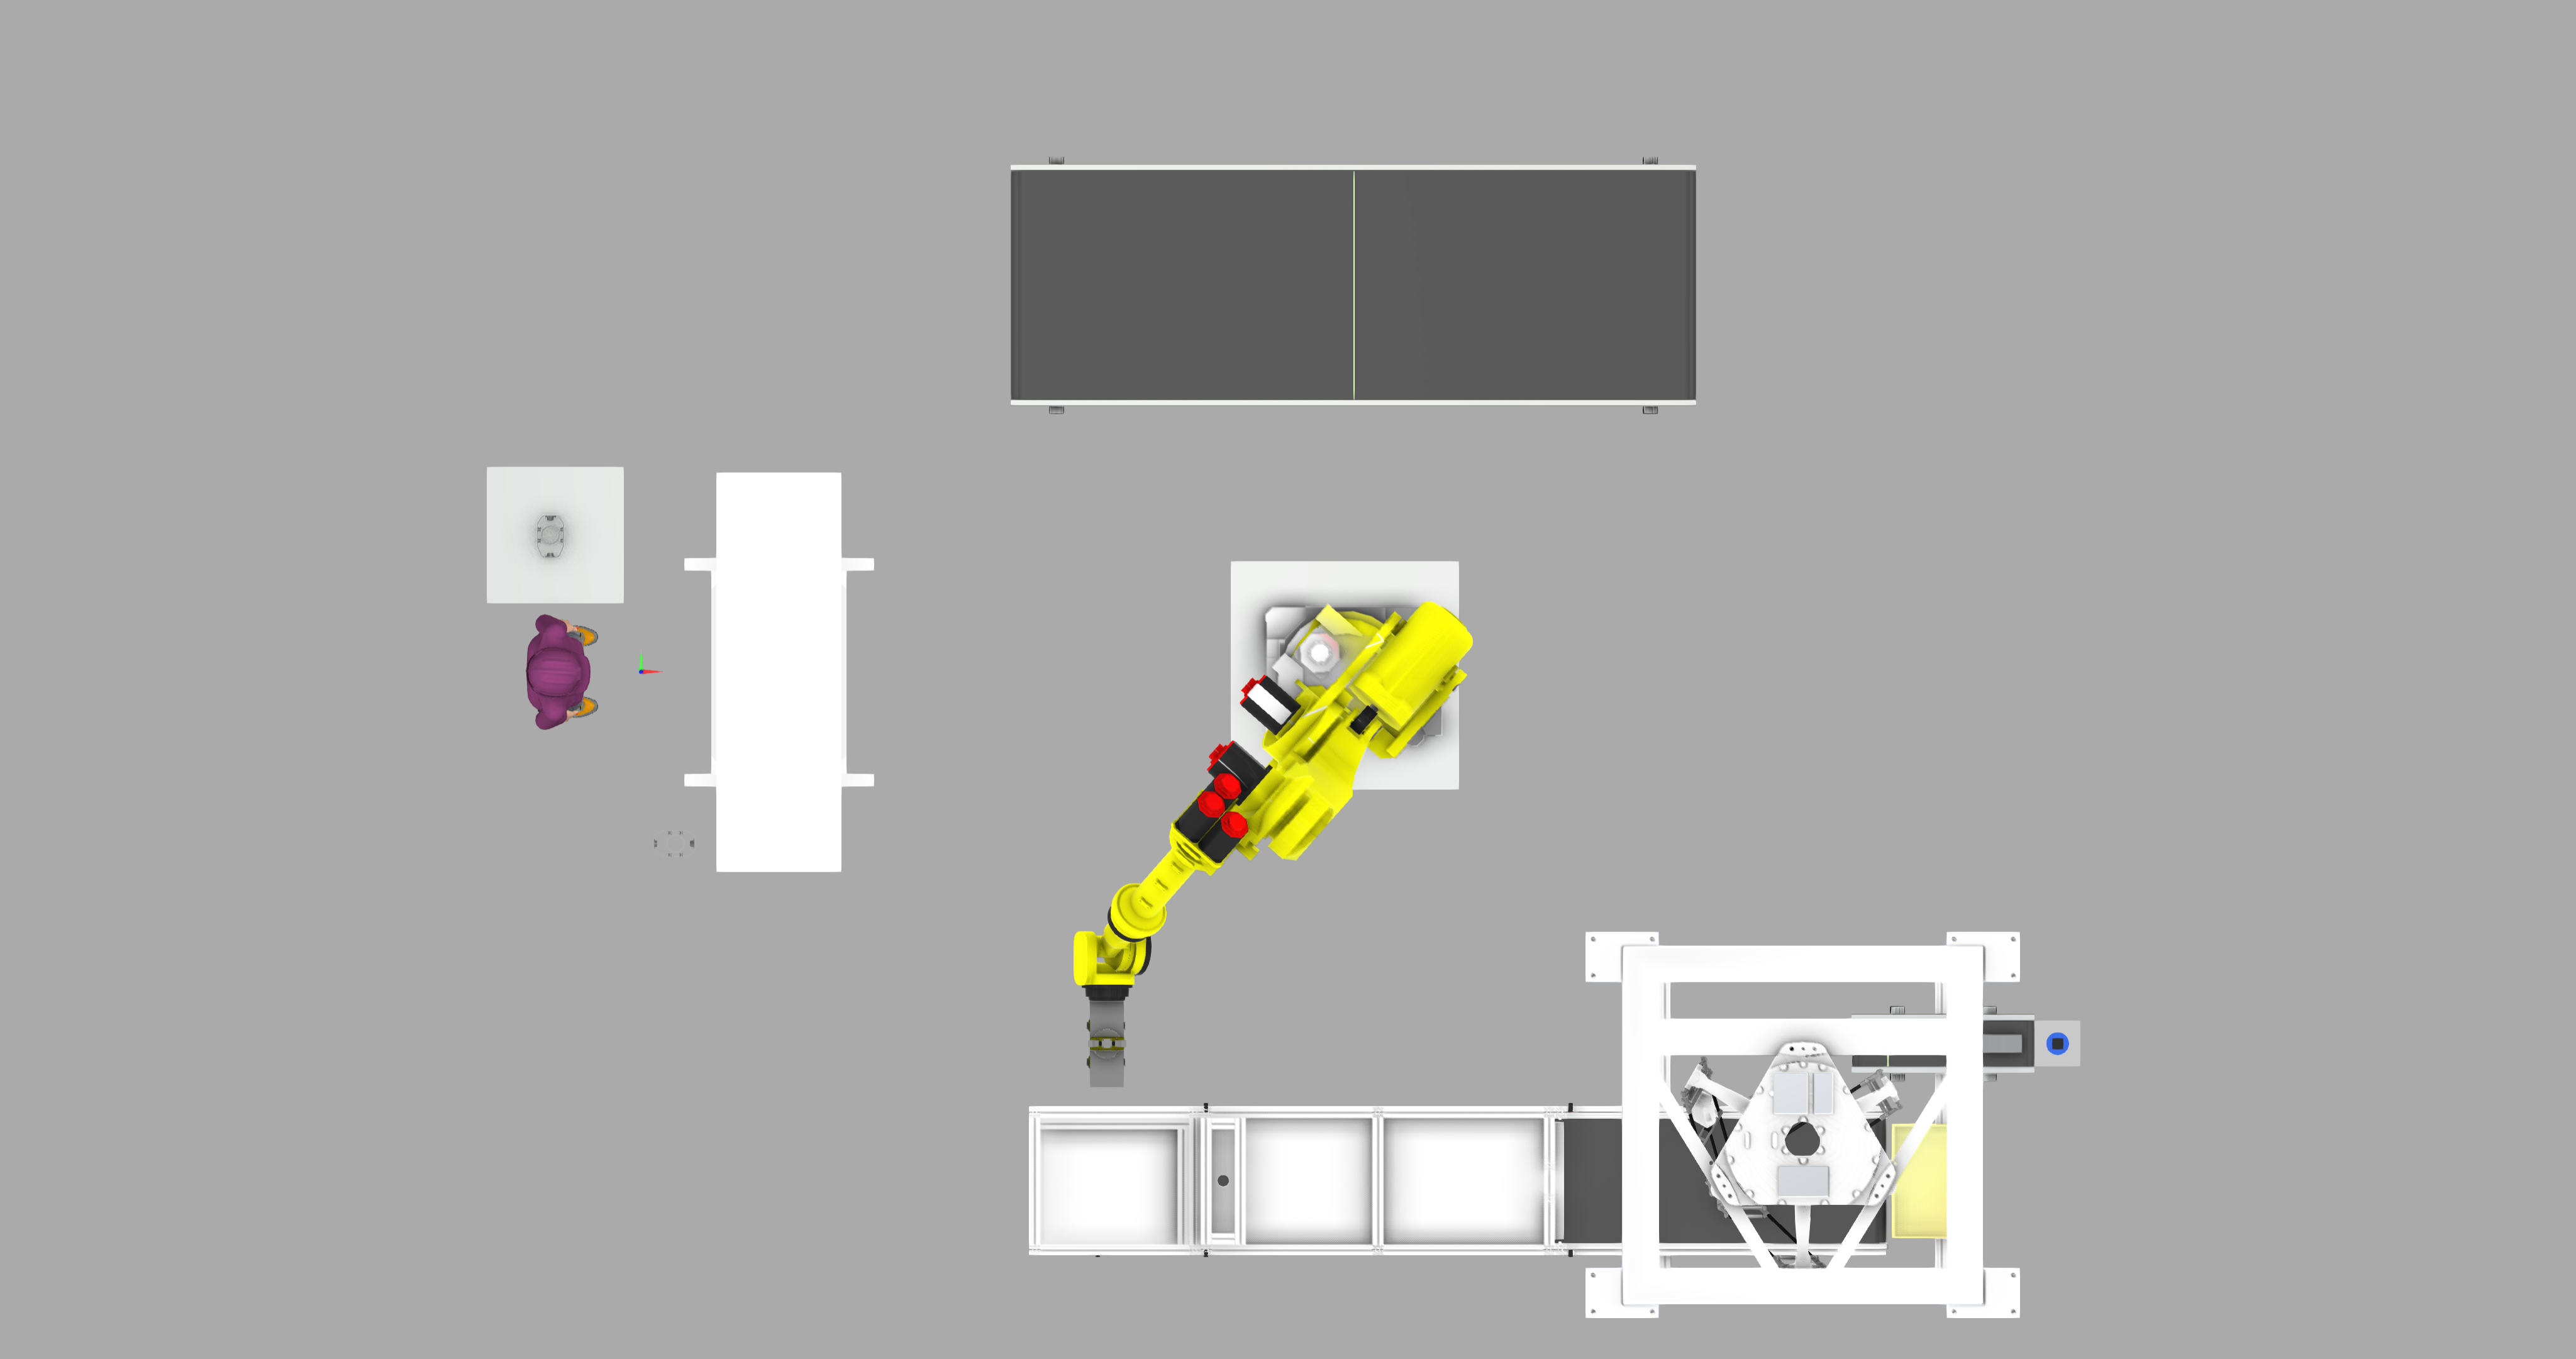
\includegraphics[
	width=\linewidth,
	center,
	keepaspectratio,
	]{ProductionLineSetup/Rendering}
	\caption{Top view of Production line layout, rendered with Visual Components \cite{AliyaThesis}}
	\label{fig:ProdLineVisComp}
\end{figure}



\paragraph{Extruder} \label{sec:extruder}
\ac{FRP} raw material pellets are fed into an extruder. 
Alternatively, reprocessed material from steps down the production line is fed into the extruder.
The extruder melts the raw material and releases it at its hot end. 
At the hot end of the extruder, the material is portioned into blops of 300g each by a guillotine.

\paragraph{Conveyor 1} \label{sec:conveyor1}
The first conveyor belt transports the \ac{FRP} material blops from the output of the \nameref{sec:extruder} to the \nameref{sec:Deltarobot}. At the end of the coveyor belt is a proximity sensor to detect incoming material.

\paragraph{Deltarobot} \label{sec:Deltarobot}
After a signal is given from the proximity sensor of \nameref{sec:conveyor1}, a  Fanuc M-3iA/6S 4-axis Delta-robot picks up the material and weighs it with a load cell built into the gripper of the robot. 
If the weight of the material is out of the desired range, it is discharged into a waste bin and recycled with the \nameref{sec:extruder}.
If the weight of the material is within an acceptable range, it is placed on \nameref{sec:conveyor2}.
When placing the material on conveyor 2, the placement position and other data are communicated to processes further down the line.
If needed, multiple blops of material can be stacked to the desired height while \nameref{sec:conveyor2} keeps moving.


\paragraph{Conveyor 2} \label{sec:conveyor2}
The second conveyor belt transports the sorted and arranged \ac{FRP} material from the \nameref{sec:Deltarobot} through the \nameref{sec:oven}. 

\paragraph{Oven}\label{sec:oven}
The oven takes in the blops of \ac{FRP} material, and brings them up to the desired temperature with induction heaters. The material is then stored in a buffer zone separated with doors from the oven and the heating chamber where the material is kept at temperature. When the \nameref{sec:HydraulicPress} is ready, a door in the buffer zone opens for the Robot arm to pick up the material.

%The oven can be separated into several zones:
%\subparagraph{Oven entrance}
%With the position data provided by the \nameref{sec:Deltarobot} and the \nameref{sec:conveyor2} speed, the oven door at the entrance can open at the right time to take in the material.
%\subparagraph{Heating chamber} \label{sec:HeatingChamber}
%In the heating chamber, the material is brought to the desired temperature with several induction heaters.
%\subparagraph{Internal door}
%With the position data provided by the \nameref{sec:Deltarobot} and the \nameref{sec:conveyor2} speed, a door inside the oven can open at the right time to take in the material.
%\subparagraph{Buffer zone} \label{sec:BufferZone}
%A buffer zone, separated from the \nameref{sec:HeatingChamber} provides an area to keep the material at the desired temperature until it can be processed further.
%\subparagraph{Oven output}
%When the \nameref{sec:HydraulicPress} is ready, a door in the \nameref{sec:BufferZone} opens for the Robot arm to pick up the material.

\paragraph{Robot arm} \label{sec:RobotArm}
The robot arm has two tasks:
\begin{enumerate}
	\item After a signal is given from the \nameref{sec:HydraulicPress}, the Fanuc 210F 6axis robot arm picks up the hot \ac{FRP} material stack from the buffer zone and places it in a \nameref{sec:HydraulicPress} with a specialized gripper. 
	After placing the part, the robot changes its gripper tool, and waits for its second task.
	\item When the forming process in the \nameref{sec:HydraulicPress} is finished, the mould opens, and the robot arm %and the same robot arm as in \nameref{sec:RobotArm1}
	can use another gripper to pick up  the \ac{FRP}-part and place it on \nameref{sec:conveyor3}.
	After placing the part, the robot changes its gripper tool, and waits for its first task
\end{enumerate}


%\paragraph{Robot arm task 1} \label{sec:RobotArm1}
%After a signal is given from the \nameref{sec:HydraulicPress}, a Fanuc 210F 6axis robot arm picks up the hot \ac{FRP} material stack from the buffer zone and places it in a \nameref{sec:HydraulicPress} with a specialized gripper.
%After placing the part, the robot changes its gripper tool, and waits for its second task, see \nameref{sec:RobotArm2}.

\paragraph{Hydraulic press} \label{sec:HydraulicPress}
After all material is placed and the \nameref{sec:RobotArm} has completely withdrawn from the press in a safe distance, the press will close the heated mould to give the \ac{FRP} material its desired shape with heat and pressure. After an estimated cycle time of 1 minute, the press opens and the finished part can be picked up.

%\paragraph{Root arm task 2} \label{sec:RobotArm2}
%When the forming process in the \nameref{sec:HydraulicPress} is finished, the mould opens, and the same robot arm as in \nameref{sec:RobotArm1} can use another gripper to pick up  the \ac{FRP}-part and place it on \nameref{sec:conveyor3}.
%After placing the part, the robot changes its gripper tool, and waits for its first task, see \nameref{sec:RobotArm1}.

\paragraph{Conveyor 3}\label{sec:conveyor3}
The third conveyor belt transports the formed part from the press to the \nameref{sec:Cobot}.

\paragraph{Cobot} \label{sec:Cobot}
When the material arrives at the cobot, it is picked up, and presented to a camera system for analysation. If the part fulfils the desired properties, it is given to further processing steps and packing.
In case, it does not fulfils the desired properties, it can be recycled with the \nameref{sec:extruder}.